%************************************************
\chapter{Diferenciación}\label{ch:01}
%************************************************

El propósito de este primer capítulo es establecer el lengüaje y notación matemática que usaremos 
en este texto. Mucho de lo que veremos es simplemente una revisión del cálcuo elemental,
especialmente diferenciación de funciones.

\section{El espacio Euclideo}

El espacio euclidiano es frecuentemente usado en matemáticas sin ser formalmente definido. Al observar la
esquina de un salón se puede ver el proceso familiar con el que se describen los ejes cartesianos y como la
medida de tres números describen la posición de un punto. Aquí, en vez de decir que tres números describen
la posición de un punto, los definimos como el punto mismo.

\begin{definition}
    $\realR^{3}$ es el conjunto de todos los pares ordenados de números reales. El par $\bm{p} = (p_{1},p_{2},p_{3})$
    es llamado un \emph{punto} de $\realR^{3}$.
\end{definition}

En álgebra lineal se muestra como $\realR^{3}$ es un espacio vectorial sobre los números reales. De hecho si
$\bm{p} = (p_{1},p_{2},p_{3})$ y $\bm{q} = (q_{1},q_{2},q_{3})$ son puntos en $\realR^{3}$, su suma es el punto

$$ \bm{p} + \bm{q} = (p_{1} + q_{1}, p_{2} + q_{2}, p_{3} + q_{3}) $$

El múltiplo escalar del punto $\bm{p}$ por un número real $a$ es el punto

$$ a\bm{p} = (ap_{1}, ap_{2}, ap_{3}) $$

Estas dos operaciones satisfacen los axiomas de un espacio vectorial. Al punto $ 0 = (0,0,0)$ lo llamamos el
\emph{origen} de $\realR^{3}$.

\begin{definition}
    Sean $x$, $y$, y $z$ funciones reales en $\realR^{3}$ tales que para cada punto $\bm{p} = (p_{1},p_{2},p_{3})$
    $$ x(\bm{p}) = p_{1}, \quad y(\bm{p}) = p_{3}, \quad z(\bm{p}) = p_{3} $$

\end{definition}

\subsection{De cuaterniones a vectores}
Los vectores como los conocemos nacieron en las primeras dos decadas del siglo IXX con la representación
geométrica de los números complejos. En 1837, William Rowan Hamilton (1805-1865) mostró que los números
complejos podian ser considerados abstractamente como pares ordenados $(a,b)$ de números reales. Esta idea
era parte de una investigación para encontrar una forma de representar "números" de dos dimensiones en tres
dimensiones, nadie logró hacerlo preservando las propiedades básicas de los reales y complejos. \\

\begin{wrapfigure}{r}{0.3\textwidth}
  \begin{center}
    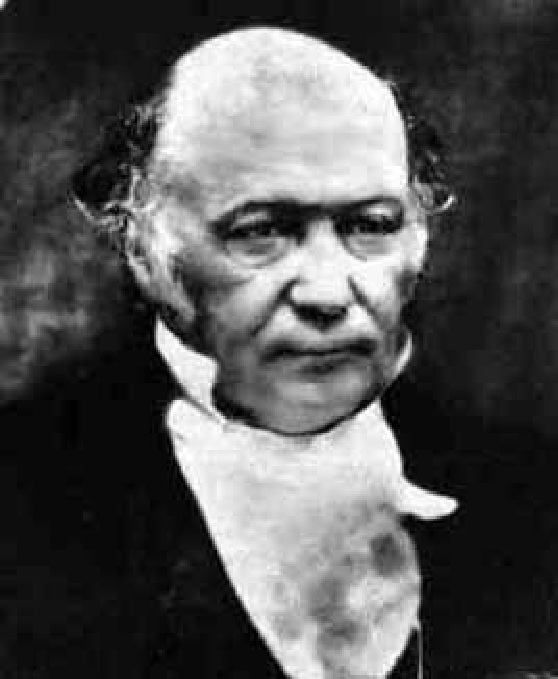
\includegraphics[width=0.3\textwidth]{gfx/hamilton}
  \end{center}
  \caption{Hamilton}
\end{wrapfigure}

Después de mucha frustración, Hamilton dejó su busqueda del tal sistema númerico de tres dimensiones e inventó
uno de cuatro dimensiones, lo llamó cuaterniones. Los cuaterniones de Hamilton se denotaban $q = w + ix + jy + kz$, donde, $w$,$x$,$y$ y $z$ eran números reales.

Aunque los cuaterniones fueron fuertemente aceptados por varios científicos, entre ellos Maxwell y Lord Kelvin,
tenian un problema que incomodaba a los matemáticos. El producto de cuaterniones no es conmutativo ni homogeneo
, es decir, $pq = -qp$.

En el tiempo que Hamilton descubrió los cuaterniones, Hermann Grassmann (1809-1867) estaba escribiendo
"The Calculus of Extension (1844)", mejor conocido por su título en alemán, Ausdehnungslehre. En 1832
Grassmann comenzó el desarrollo de un nuevo cálculo geométrico y subsecuentemente usó este estudio para
simplificar porciones de dos trabajos clásicos, Analytical Mechanics de Joseph Louis Lagrange y Celestial
Mechanics de Pierre Simon Laplace. En su libro, Grassmann por primera vez expande la idea del concepto
de un vector (como $ix + jy + kz$ de los cuaterniones) de dos a tres y $n$ dimensiones, lo cual expandios
la idea de dimensión de un espacio.

\begin{wrapfigure}{l}{0.3\textwidth}
  \begin{center}
    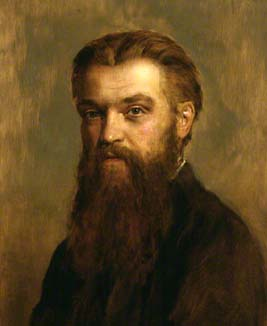
\includegraphics[width=0.3\textwidth]{gfx/clifford}
  \end{center}
  \caption{Clifford}
\end{wrapfigure}

William Kingdon Clifford (1845 - 1879) expresó profunda admiración por la obra de Grassmann, y claramente
favoreció a los vectores sobre los cuaterniones. Clifford separó el producto de dos cuaterniones en dos
productos diferentes de vectores, los cuales llamó producto escalar y producto vectorial, solucionando
el problema del producto de cuaterniones.

El desarrolo del álgebra de vectores y análisis vectorial como lo conocemos hoy día fue descrito en un conjunto
de notas por el matemático J. Williard Gibbs (1839-1903) para sus estudiantes de la Universidad de Yale.

\clearpage


\section{Límites y continuidad}

Esta sección está centrada en los conceptos de conjunto abierto, límite y continuidad; los conjuntos abiertos son necesarios para entender los límites y, a su vez, los límites son necesarios para entender continuidad y diferenciabilidad.

\begin{figure}[!ht]
  \begin{center}
      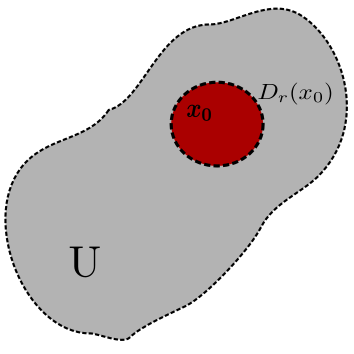
\includegraphics[width=0.5\linewidth]{gfx/conjunto-abierto}
      \caption{}
      \label{fig:boat1}
  \end{center}
\end{figure}

Además establecemos la convención de que el conjunto vacio $\emptyset$ es abierto.

\begin{theorem}
    Para cada $\bm{x_{0}} \in \realR^{n}$ y $r > 0$, $D_{r}(\bm{x_{0}})$ es un conjunto abierto.
\end{theorem}

\begin{proof}
    Sea $\bm{x} \in D_{r}(\bm{x_{0}})$, esto es, sea $\|\bm{x} - \bm{x_{0}}\| < r$. De acuerdo con la definición
    de conjunto abierto, debemos hallar un $s > 0$ tal que $D_{s}(\bm{x}) \subset  D_{r}(\bm{x_{0}})$.
    Sea $s = r - \|\bm{x} - \bm{x_{0}}\|$, nótese que $s > 0$, pero que $s$ se hace más chico si $\bm{x}$ está
    cerca del borde $D_{r}(\bm{x_{0}})$ \\

    Para probar que $D_{s}(\bm{x}) \subset D_{r}(\bm{x_{0}})$, sea $\bm{y} \in D_{s}(\bm{x})$; esto es, sea
    $\|\bm{y} - \bm{x}\| < s$. Queremos probar que también $\bm{y} \in D_{r}(\bm{x_{0}})$. Probar esto en vista
    de la definición de un r-disco, equivale a demostrar que $\|\bm{y} -\bm{x_{0}}\| < r$. Usemos la desigualdad
    del triángulo para esto

    \begin{eqnarray*}
        \|\bm{y} - \bm{x_{0}}\| &=& \|(\bm{y} - \bm{x}) + (\bm{x} - \bm{x_{0}})\| \\
                              &\le& \|\bm{y} - \bm{x}\| + \|\bm{x} - \bm{x_{0}}\| \\
                              &=& r
    \end{eqnarray*}

    De aquí que $\|\bm{y} - \bm{x_{0}}\| < r$. \qed

\end{proof}

\begin{definition}
    Sea $A \subset \realR^{n}$ es punto frontera de $A$ si toda vecindad de $\bm{x}$ contiene al menos un punto de $A$ y al menos un punto fuera de $A$.
\end{definition}

En esta definición, $\bm{x}$ puede estar o no en $A$; si $\bm{x} \in A$, entonces $\bm{x}$ es un punto frontera si toda vecindad de $\bm{x}$ contiene al menos un punto
que no esté en $A$. De manera análoga, si $\bm{x}$ no está en $A$, es un punto frontera si toda vecindad de
$\bm{x}$ contiene al menos un punto de $A$.

\begin{figure}[!ht]
  \begin{center}
      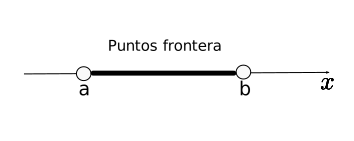
\includegraphics[width=0.5\linewidth]{gfx/puntos-frontera}
      \caption{}
      \label{fig:boat1}
  \end{center}
\end{figure}


Ya estamos en posición de definir un límite. Durante toda la exposición siguiente, el dominio de definición de la función $f$ será un conjunto abierto $A$.
Nos interesa hallar el límite de $f$ cuando $\bm{x} \in A$ tienda a un punto de $A$ o a un punto frontera de $A$.

El concepto de límite es una herramienta básica y útil para el análisis de funciones; nos permite estudiar derivadas y de especial interes en este texto,
derivadas parciales.

\begin{definition}[Límite]
    Sea $f:A \subset \realR^{n} \mapsto \realR^{m}$, donde $A$ es un conjunto abierto. Sea $\bm{x_{0}}$ un punto de $A$ o en la frontera de $A$, y sea
    $V$ una vecindad de $\bm{b} \in \realR^{m}$. Decimos que $f$ está en $V$ conforme $\bm{x}$ tiende a $\bm{x_{0}}$ si existe una vecindad $U$ de 
    $\bm{x_{0}}$ tal que $\bm{x} \neq \bm{x_{0}}$, $\bm{x} \in U$ y $\bm{x} \in A$ implica $f(x) \in V$. Decimos que $f(x)$ tiende a $\bm{b}$ cuando
    $\bm{x}$ tiende a $\bm{x_{0}}$, es decir

    $$ \lim_{\bm{x} \rightarrow \bm{x_{0}}} f(x) = b $$
\end{definition}

Del cálculo de una variable sabemos que el concepto de función continua está basado en la idea intuitiva de una función cuya gráfica es una
curva sin romper, esto es, una curva sin saltos (una curva suave).

\{ Añadir ejemplos de funciones continuas y no continuas \}

\begin{definition}
    Sea $f:A \subset \realR^{n} \mapsto \realR^{m}$ una función dada con dominio $A$. Sea $\bm{x_{0}} \in A$. Decimos que $f$ es continua
    en $\bm{x_{0}}$ si y sólo si
    $$ \lim_{\bm{x} \rightarrow \bm{x_{0}}} f(\bm{x}) = f(\bm{x_{0}})$$
\end{definition}

\section{Derivadas Parciales}

%*****************************************




